\documentclass{article}
\usepackage{graphicx} % Required for inserting images
\usepackage[T2A]{fontenc}
\usepackage[english, russian]{babel}

\setlength\parindent{1.5em}


\title{Домашнее задание 1}
\author{Андрей Зотов}
\date{Апрель 2023}

\begin{document}

\maketitle

\section*{Задача 1.а}
{\bf Ответ:} равенство $A\setminus (A\cap B)= A \cap(A \setminus B)$ выполнено для любых $A$ и $B$.
\\
\\
{\bf Доказательство.} Из диаграммы Эйлера-Венна (ниже) видно, что с одной стороны $A\setminus (A\cap B) = A\setminus B$, а с другой стороны $A \cap(A \setminus B) = A\setminus B$. Т.е. левая и правая части доказываемого равенства равны.
\\
{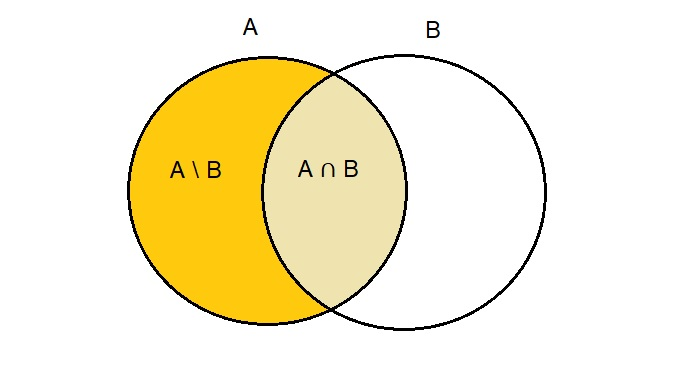
\includegraphics[scale=0.8]{img/img1.jpg}}
\section*{Задача 1.б}
{\bf Ответ:} равенство $(A\cup B)\triangle (A\cap B)= A \triangle B$ выполнено для любых $A$ и $B$.
\\
\\
{\bf Доказательство.} По определению симметрической разницы $(A\cup B)\triangle (A\cap B) = ((A\cup B)\setminus(A\cap B))\cup((A\cap B)\setminus (A\cup B))$. При этом из диаграммы Эйлера-Венна (ниже) видно, 
что $(A\cup B)\setminus(A\cap B) = A \triangle B$ и $(A\cap B)\setminus (A\cup B) =  \emptyset$, т.е. левая часть равенства равна $(A \triangle B) \cup  \emptyset$, которая в свою очередь равна правой части равенства $A \triangle B$. Что и требовалось доказать.
\\
{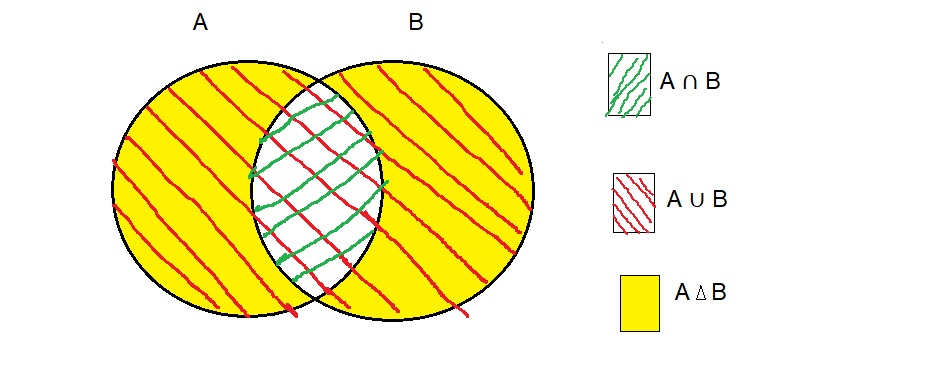
\includegraphics[scale=0.8]{img/img2.jpg}}
\section*{Задача 1.в}
{\bf Ответ:} равенство $((A \setminus B) \cup(A \setminus C)) \cap(A \setminus(B \cap C))=A \backslash(B \cup C)$, вообще говоря, выполняется не для любых $A,B$ и $C$. Контрпример: $B = \emptyset$, $A=\{a,b\}$, $C=\{a\}$
\\
\\
{\bf Доказательство.} На диаграммах Эйлера-Венна (1 и 2), наглядно видно, что  $(A \backslash B) \cup(A \backslash C) = A \backslash(B \cap C)$. Обозначим желтую область диаграмм 1 и 2 как $F$. Таким образом, левая часть равенства будет $F\cap F = F$ . При этом на диаграмме 3 видно, что правая часть равенства (область закрашенная желтым), вообще говоря, отличается от $F$.
\par
Видя эти диаграммы, нетрудно подобрать контрпример: пусть $B=\emptyset$, тогда $(A \backslash B) \cup(A \backslash C) = A $, т.е. левая часть будет $F = A$, в то же время  правая часть будет $A \setminus(\emptyset \cup C) = A \setminus C$, т.е. не совпадает с левой частью, если $A\cap C \neq \emptyset$. Т.е. контрпример может быть, например, таким: $B = \emptyset$, $A=\{a,b\}$, $C=\{a\}$ - в этом случае элемент $a$ входит в левую часть, а в правую не входит.
\\
{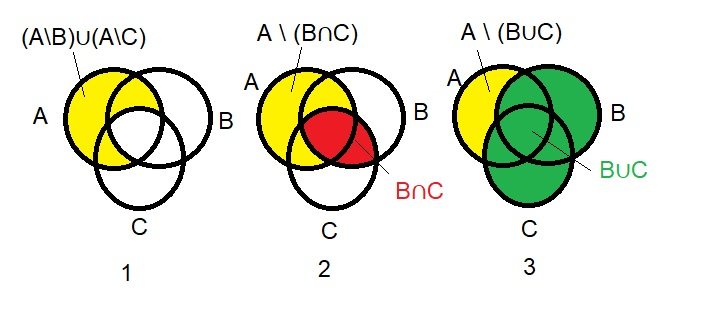
\includegraphics[scale=0.8]{img/img3.jpg}}
\section*{Задача 2}
{\bf Ответ:} утверждение верно. Для любых множеств $A$ и $B$ выполняется включение
$$(A\cup B)\setminus B \subseteq A$$
{\bf Доказательство.} На диаграмме (ниже) наглядно видно, что множество $(A\cup B)\setminus B = A\setminus B$ и, очевидно, является подмножеством $A$. Что и требовалось показать.
\\
{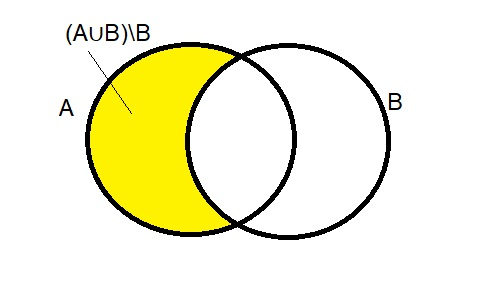
\includegraphics[scale=0.8]{img/img4.jpg}}
\section*{Задача 3}
{\bf Решение.} Пусть $\varphi_1(a, b) = \neg (a\vee (b \oplus 1))\wedge (a \rightarrow 1)$ и $\varphi_2(a, b) = \neg a \wedge b$. Тогда учитывая, что $a \rightarrow 1 \equiv 1$,  $x \wedge 1 \equiv x$ и $b \oplus 
 1 \equiv \neg b$ , получаем $\varphi_1(a, b) = \neg (a\vee \neg b)$. Раскрывая эту скобку по закону де Моргана, и учитывая что $\neg \neg b \equiv b$, получаем $\varphi_1(a, b) =  \neg a \wedge b = \varphi_2(a, b)$. Что и требуется.
 \\
 \section*{Задача 4}
 {\bf Ответ:} высказывание ложно в случаях б), в) и г).
 \\
 \\
 {\bf Решение.} Если $x$ некоторое число, то высказывание из условия можно представить как предикат:
 $$P(x) = Q(x) \wedge ( R(x) \rightarrow \neg S(x) )$$
 где
 \begin{itemize}
     \item $Q(x) = $ "Число $x$ четно"
     \item $R(x)=$ "В числе $x$ 7 цифр"
     \item $S(x)=$ "Третий разряд числа $x$ четный"
 \end{itemize}
 Тогда:
 \begin{itemize}
 \item а) если $x = 0 \Rightarrow Q(x) = 1, R(x) = 0, S(x) = 1$  $\Rightarrow$ $P(x) = 1 \wedge (0\rightarrow\neg 1)=1$
 \item б) если $x=1234567\Rightarrow Q(x)=0,R(x)=1,S(x)=0\Rightarrow P(x)=0 \wedge (1\rightarrow\neg 0)=0$
 \item в) если $x=2222222\Rightarrow Q(x)=1,R(x)=1,S(x)=1\Rightarrow P(x)=1\wedge(1\rightarrow\neg 1)=0$
 \item г) если $x=123457\Rightarrow Q(x)=0,R(x)=0,S(x)=1\Rightarrow P(x)=0\wedge(0\rightarrow\neg 1)=0$
 \end{itemize}
 Таким образом высказывание ложно в случаях б), в) и г).
\section*{Задача 5}
{\bf Ответ:} $x\in\{0, 1, 3, 5, 7, 8, 9\}$
 \\
 \\
{\bf Решение.} Множество $A$ - это натуральные числа от 1 до 7 включительно - $\{1,2,3,4,5,6,7\}$. Множество $B$ - это множество всех четных целых чисел. Множество $C$ - это множество всех целых чисел от 0 до 9 включительно - $\{0,1,2,3,4,5,6,7,8,9\}$. Поэтому предикат $Q(x) = \neg(x \in B)$ обращается в истину тогда и только тогда, когда $x$ не является четным.
\par
Множество $C$ можно разложить на два непересекающихся множества - первое состоит из элементов, которые входят в $A$, а второе из элементов, которые не входят в $A$. Поэтому рассмотрим 2 случая:
\begin{itemize}
    \item 1) $x\in A\cap C = \{1,2,3,4,5,6,7\}$. Для этих $x$ предикат $P(x) = (x\in A)$ обращается в истину, поэтому чтобы предикат $P(x)\rightarrow Q(x)$ обращался в истину необходимо, чтобы $Q(x)$ был истиной, а это возможно только когда $x$ не является четным числом, т.е. при $x\in \{1,3,5,7\}$
    \item  2) $x\in C\setminus A=\{0,8,9\}$. Для этих $x$ предикат $P(x)$ ложен, поэтому значение $Q(x)$, вообще говоря, не важно (т.к. $0\rightarrow x\equiv 1$), т.е. предикат $P(x)\rightarrow Q(x)$ обращается в истину при $x\in\{0,8,9\}$.
\end{itemize}
\par
Таким образом, объединяя два этих множества подходящих $x$, получаем, что предикат $P(x)\rightarrow Q(x)$ обращается в истину для $x\in C$, если  $x\in\{0,1,3,5,7,8,9\}$.
\section*{Задача 6}
{\bf Доказательство.} Докажем утверждение по индукции. База индукции выполняется: при $n=1$ утверждение верно: $2 = 1 * 2$. Докажем теперь шаг индукции. 
Пусть утверждение верно для $n=k$, т.е. верно, что: $$2+4+\dots+2k=k(k+1)$$
Тогда при $n=k+1$ получаем: $$2+4+\dots+2k+2(k+1)=k(k+1)+2(k+1)=(k+1)(k+2)$$
Т.е. утверждение верно для $n=k+1$ в предположении, что оно верно для $n=k$. Шаг индукции доказан.  Таким образом утверждение доказано по индукции.

\end{document}
